\chapter{連立一次方程式の解法}
\label{app:linear-systems}

第2章では \texttt{numpy.linalg.solve}、付録\ref{app:axisym-poisson}では \texttt{scipy.sparse.linalg.spsolve} を使い、
Poisson 方程式を離散化して得た連立一次方程式を解いた。
本付録は、その求解の仕組みを確認するための背景資料である。
同じ小さな連立一次方程式を使い、Gauss の消去法、LU 分解、疎行列の消去、Jacobi 法を順に説明する。
行列の構造と解法の種類を区別し、計算結果を残差でどう確認するかを学ぶ。
数値計算法は幸谷第7・8章\cite{kouya2021}を参考にする。

本編と同様に、一般的なソルバーの自作は求めない。
以下では $m$ 個の未知数に対する正方行列の問題 $A\boldsymbol u=\boldsymbol b$ を扱い、解は一意に定まるとする。
式と実装の対応は短い Listing で示す。付録D専用の Notebook は設けず、Notebook 2末尾の補足「付録D：連立一次方程式の解法」も参照できる。

\section{Gauss の消去法：小さな例}
\label{sec:appD-elimination}

第2章の三重対角行列と同じ構造を持つ、説明用の例を考える。
ここでは計算手順を追うため、右辺を $\boldsymbol b=(1,0,1)^{\mathsf T}$ と選ぶ。
この右辺は Plummer 球の密度や境界値から求めたものではない。連立一次方程式は
\begin{equation}
 \underbrace{\begin{pmatrix}2&-1&0\\-1&2&-1\\0&-1&2\end{pmatrix}}_{A}
 \begin{pmatrix}u_1\\u_2\\u_3\end{pmatrix}
 =\begin{pmatrix}1\\0\\1\end{pmatrix}
\label{eq:appD-example}
\end{equation}
である。これは、$2u_1-u_2=1$、$-u_1+2u_2-u_3=0$、$-u_2+2u_3=1$ の3式をまとめたものである。

一つの式の定数倍を別の式に加える操作は、同じ定数倍を引けば元に戻せるため、解を変えない。
この操作で未知数を順番に消す方法を\textbf{Gauss の消去法（Gaussian elimination）}と呼ぶ。
係数と右辺を縦線で区切って並べ、$R_i$ を第 $i$ 行と書くと、まず
\begin{equation}
 \left[\begin{array}{ccc|c}2&-1&0&1\\-1&2&-1&0\\0&-1&2&1\end{array}\right]
 \xrightarrow{\ R_2\leftarrow R_2+\frac12R_1\ }
 \left[\begin{array}{ccc|c}2&-1&0&1\\0&\frac32&-1&\frac12\\0&-1&2&1\end{array}\right]
\label{eq:appD-first-elimination}
\end{equation}
として、第2行の $u_1$ を消す。次に、\textbf{更新後の第2行}を使って
\begin{equation}
 R_3\leftarrow R_3+\frac23R_2
 \quad\Longrightarrow\quad
 \left[\begin{array}{ccc|c}2&-1&0&1\\0&\frac32&-1&\frac12\\0&0&\frac43&\frac43\end{array}\right]
\label{eq:appD-second-elimination}
\end{equation}
とすると、第3行の $u_2$ も消える。
このように対角成分より下を0にする操作が\textbf{前進消去（forward elimination）}である。
係数だけを変えると別の連立方程式になるため、右辺にも同じ行操作を行う。

得られた上三角の連立方程式は、下の行から順に解ける。
\begin{equation}
 u_3=\frac34\cdot\frac43=1,\qquad
 u_2=\frac23\left(\frac12+u_3\right)=1,\qquad
 u_1=\frac{1+u_2}{2}=1.
\label{eq:appD-back-substitution}
\end{equation}
この操作を\textbf{後退代入（back substitution）}と呼ぶ。
求めた解 $\boldsymbol u=(1,1,1)^{\mathsf T}$ を式\eqref{eq:appD-example}へ代入すると、元の3式を満たす。
\textbf{前進消去で解きやすい形に変え、後退代入で解を求める}のが基本である。

第2章と同じライブラリでこの例を解き、元の方程式に代入して確認するコードを Listing D.1に示す。
この例では厳密解が分かるので、残差だけでなく解そのものの誤差も計算できる。

\begin{listingbox}[left=6mm]{D.1　小さな連立一次方程式の求解と検証}
\begin{Verbatim}[fontsize=\small]
import numpy as np

A = np.array([[2.0, -1.0, 0.0], [-1.0, 2.0, -1.0], [0.0, -1.0, 2.0]])
b = np.array([1.0, 0.0, 1.0])
u_num = np.linalg.solve(A, b)

# 元の方程式の残差と、既知の厳密解からの誤差を別々に調べる
residual_max = np.max(np.abs(A @ u_num - b))
solution_error = np.max(np.abs(u_num - np.ones(3)))
\end{Verbatim}
\end{listingbox}

有限精度の計算では、解が見かけ上 $(1,1,1)$ と表示されても、残差が厳密に0になるとは限らない。
残差と解の誤差の違いは、\ref{sec:appD-iterative}節でも確認する。

\section{LU 分解：消去手順の行列表現}
\label{sec:appD-lu}

前節の行列 $A$ は、次の二つの三角行列の積に分解できる。
\begin{equation}
 \boxed{A=LU},\qquad
 L=\begin{pmatrix}1&0&0\\-\frac12&1&0\\0&-\frac23&1\end{pmatrix},\qquad
 U=\begin{pmatrix}2&-1&0\\0&\frac32&-1\\0&0&\frac43\end{pmatrix}.
\label{eq:appD-lu}
\end{equation}
$L$ は対角成分より上が0の下三角行列、$U$ は対角成分より下が0の上三角行列である。
ここでは $L$ の対角成分をすべて1に取っている。
この分解を\textbf{LU 分解（LU decomposition）}と呼ぶ。
$U$ は前進消去の結果で、$L$ には消去に使った倍率が記録されている。
例えば第2行の消去は $R_2\leftarrow R_2-\ell_{21}R_1$ と書け、
$\ell_{21}=-1/2$ である。これが $L$ の第2行・第1列の値になる。
同様に、更新後の第2行を使う倍率 $\ell_{32}=-2/3$ が $L$ に入る。

$A\boldsymbol u=\boldsymbol b$ に $A=LU$ を代入し、$\boldsymbol y=U\boldsymbol u$ とおけば、
\begin{equation}
 \underbrace{L\boldsymbol y=\boldsymbol b}_{\text{上の行から解く}}
 \qquad\longrightarrow\qquad
 \underbrace{U\boldsymbol u=\boldsymbol y}_{\text{下の行から解く}}
\label{eq:appD-triangular-solves}
\end{equation}
の2段階になる。下三角系を上から解く操作が\textbf{前進代入（forward substitution）}である。
本例では
\begin{equation}
 y_1=1,\qquad
 y_2=0+\frac12y_1=\frac12,\qquad
 y_3=1+\frac23y_2=\frac43
\label{eq:appD-forward-substitution}
\end{equation}
となり、$\boldsymbol y$ は式\eqref{eq:appD-second-elimination}の変形後の右辺に一致する。
あとは前節と同じ後退代入で $\boldsymbol u$ を求める。
\textbf{前進消去は行列を変形する操作、前進代入は下三角系を解く操作}である。

同じ $A$ に対して右辺 $\boldsymbol b$ だけが変わる場合、一度求めた $L,U$ を再利用できる。
各右辺について前進代入と後退代入だけを行えばよいことが、LU 分解の利点である\cite{kouya2021}。
第2章の Poisson 方程式でも、格子と差分式を固定して密度や境界値だけを変えるなら、係数行列は変わらず右辺だけが変わる。
ただし、格子を変える収束試験では行列も変わるので、同じ分解をそのまま使うことはできない。

\subsection{行を入れ替える場合}
一般の行列では、解が一意に定まっていても、消去の途中で割る成分が0になることがある。
0でなくても、他の成分に比べて小さい値で割ると、丸め誤差が増幅される場合がある。
この割る成分を\textbf{枢軸（pivot、ピボット）}という。
\textbf{部分枢軸選択（partial pivoting）}では、処理する列の未処理部分から絶対値が最大の成分を選び、
その行を現在の行と入れ替える。右辺も同じ順に入れ替える。
行の入れ替えを表す行列を $P$ と書けば、本書の記法では
\begin{equation}
 PA=LU,\qquad L\boldsymbol y=P\boldsymbol b,\qquad U\boldsymbol u=\boldsymbol y
\label{eq:appD-pivot-lu}
\end{equation}
となる。行を入れ替えても未知数の順番は変わらない。
本例では行交換は不要である\cite{kouya2021}。

\subsection{なぜ逆行列を作らずに \texttt{solve} を使うのか}
数学的には $\boldsymbol u=A^{-1}\boldsymbol b$ と書けるが、解だけが必要なら逆行列全体を作る必要はない。
逆行列を求めてから右辺を掛ける方法は、LU 分解と代入で解く方法より計算量が増える\cite{kouya2021}。
第2章と Listing D.1の \texttt{np.linalg.solve(A, b)} も、逆行列を明示的に作るのではなく、LU 分解を用いて解を求める。

消去法や LU 分解のように、所定の消去・代入で解を求める方法を\textbf{直接法（direct method）}と呼ぶ。
ただし、計算機では丸め誤差があるため、「直接法」は「誤差がない方法」という意味ではない。

\section{疎行列の消去と代入}
\label{sec:appD-sparse}

付録\ref{app:axisym-poisson}で定義した「疎行列」は、0の要素が多いという\textbf{行列の構造}を表し、解法の名前ではない。
疎行列にも前節の LU 分解を使える。
違いは、0の要素まで一律に保存・計算するのではなく、\textbf{必要な非零要素を扱いながら消去と代入を進める}ことである。
まず前節と同じ三重対角系で、その計算を具体的に見る。

\subsection{三重対角行列と Thomas 法}

式\eqref{eq:appD-example}の行列では、第1列で消す必要があるのは第2行の $-1$ だけである。
第3行の第1成分は初めから0なので、第1行を使って第3行を更新する必要はない。
第2列でも、更新するのは第3行だけである。

この行列を、対角が2、隣接する副対角が $-1$ の $m$ 次三重対角行列へ拡張する。
未知数は $u_1,\ldots,u_m$ で、両端の式には範囲外の未知数を含めない。
消去後の第 $i-1$ 行が
\begin{equation*}
 d_{i-1}u_{i-1}-u_i=y_{i-1}
\end{equation*}
になったとする。次の行 $-u_{i-1}+2u_i-u_{i+1}=b_i$ に、その $1/d_{i-1}$ 倍を加えると、
\begin{equation}
 \left(2-\frac{1}{d_{i-1}}\right)u_i-u_{i+1}
 =b_i+\frac{y_{i-1}}{d_{i-1}}
\label{eq:appD-sparse-row}
\end{equation}
となり、$u_{i-1}$ が消える。つまり、更新が必要なのは対角成分と右辺だけである。
\begin{equation}
 d_1=2,\quad y_1=b_1,\qquad
 d_i=2-\frac{1}{d_{i-1}},\quad
 y_i=b_i+\frac{y_{i-1}}{d_{i-1}}\quad(i=2,\ldots,m).
\label{eq:appD-tridiagonal-forward}
\end{equation}
最後の行には $u_{m+1}$ がないので $d_mu_m=y_m$ である。下の行から
\begin{equation}
 u_m=\frac{y_m}{d_m},\qquad
 u_i=\frac{y_i+u_{i+1}}{d_i}\quad(i=m-1,\ldots,1)
\label{eq:appD-tridiagonal-back}
\end{equation}
と代入すれば解が得られる。

前節の $\boldsymbol b=(1,0,1)^{\mathsf T}$ では、計算する数は次のとおりである。
\begin{table}[H]
\centering
\caption{3未知数の例で、前進消去により更新される対角成分と右辺。}
\label{tab:appD-thomas}
\renewcommand{\arraystretch}{1.25}
\begin{tabular}{ccl}
\toprule
行 $i$ & 消去後の対角 $d_i$ & 消去後の右辺 $y_i$ \\
\midrule
1 & $2$ & $1$ \\
2 & $2-1/2=3/2$ & $0+1/2=1/2$ \\
3 & $2-1/(3/2)=4/3$ & $1+(1/2)/(3/2)=4/3$ \\
\bottomrule
\end{tabular}
\end{table}
これは式\eqref{eq:appD-second-elimination}と同じ結果である。
式\eqref{eq:appD-tridiagonal-back}から、再び $u_3=u_2=u_1=1$ を得る。
新しい解法へ置き換えたのではなく、\textbf{同じ消去法から0に対する不要な操作を省いている}。

三重対角行列の非零要素は $3m-2$ 個である。この例では各行を1回ずつ消去・代入するため、演算回数と記憶量は $m$ に比例する。
このように三重対角系の構造を利用して前進消去と後退代入を行う手順は、\textbf{Thomas 法（Thomas algorithm）}と呼ばれる。

この例では、式\eqref{eq:appD-tridiagonal-forward}から
\begin{equation}
 d_i=\frac{i+1}{i}>0\qquad(i=1,\ldots,m)
\label{eq:appD-positive-pivots}
\end{equation}
となる。実際、$d_{i-1}=i/(i-1)$ を漸化式に代入すれば $d_i=(i+1)/i$ を得る。
したがって、この係数行列では0で割ることはない。
一般の三重対角行列では、係数に応じて漸化式が変わり、消去中に割る成分が0または非常に小さくなる場合もある。
三重対角という構造だけで、行交換なしの消去が常に使えるわけではない。

\subsection{一般の疎行列とフィルイン}

三重対角の例では、消去後も隣接した成分だけを扱えた。
一方、付録\ref{app:axisym-poisson}のような2次元の問題では、消去によって最初は0だった位置にも非零の値が生じる。
ここでは、両方向の格子幅を $h$ とする直交格子で、2行2列の内部点を行ごとに番号付けした4未知数の例を使う。
2次元 Poisson 方程式の5点差分式に $-h^2$ を掛け、既知の境界値を右辺へ移すと、係数行列は次の形になる。
\begin{equation}
 B=\begin{pmatrix}
 4&-1&-1&0\\
 -1&4&0&-1\\
 -1&0&4&-1\\
 0&-1&-1&4
 \end{pmatrix}
\label{eq:appD-sparse2d-example}
\end{equation}
付録\ref{app:axisym-poisson}の軸対称系とは係数が異なるが、隣接点が結び付く構造は共通である。

第1列を消すために $R_2\leftarrow R_2+\frac14R_1$ とすると、第2行は
\begin{equation}
 (-1,4,0,-1)+\frac14(4,-1,-1,0)
 =\left(0,\frac{15}{4},-\frac14,-1\right)
\label{eq:appD-fill-example}
\end{equation}
へ変わる。\textbf{第2行・第3列の0が $-1/4$ に変わった。}
このように消去で新たに生じる非零要素を\textbf{フィルイン（fill-in）}と呼ぶ。
疎行列の直接法でも、この成分を無視してよいわけではなく、保存して以後の計算に使う。


図\ref{fig:appD-sparse-fill-in}は、二つの例について前進消去の前後の非零要素の位置を比較したものである。
三重対角行列では新たな非零位置は生じないが、行列 $B$ では上三角行列 $U_B$ の第2行・第3列にフィルインが残る。
フィルインとは、元は0だった位置に値が生じることを指す。下三角部分を消しているため、図の前後で非零要素の総数が増えるとは限らない。

\begin{figure}[H]
\centering
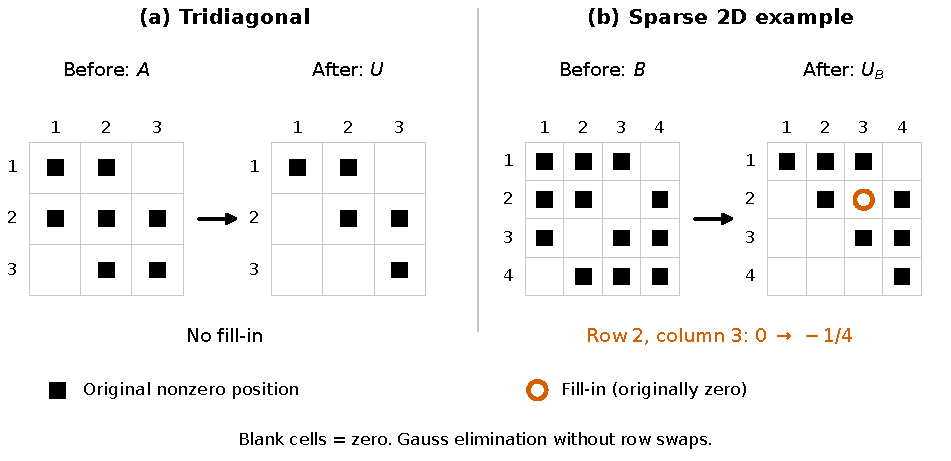
\includegraphics[width=\linewidth]{appD_sparse_elimination_fillin.pdf}
\caption{疎行列の前進消去と新たに生じる非零要素（フィルイン）。行交換を行わず、(a) 式\eqref{eq:appD-example}の $A$ と消去後の $U$、
(b) 式\eqref{eq:appD-sparse2d-example}の $B$ と消去後の $U_B$ を比較している。
黒い四角は元の行列でも非零だった位置、朱色の白抜き丸は元は0だった位置に生じた非零要素を表し、空白は0である。
(b) の第2行・第3列の値は、式\eqref{eq:appD-fill-example}で求めた $-1/4$ である。
記号は非零の位置だけを表し、係数の大きさや符号は表していない。}
\label{fig:appD-sparse-fill-in}
\end{figure}

図\ref{fig:appD-sparse-fill-in}に示したのは $U$ の非零位置だけであり、実際の LU 分解では $L$ も保存する。
必要な記憶量は、元の行列の非零要素数だけでは決まらない。
疎行列の LU 分解では、非零要素の位置を管理しながら消去を行い、得られた三角行列に前進代入と後退代入を行う。
非零要素の増加を抑えるために未知数の順を並べ替え、数値的な安定性のために行を入れ替えることもある。
\textbf{基本はあくまで LU 分解と代入であり、疎な構造に合わせて計算と保存の方法を工夫している。}

\subsection{第2章の \texttt{solve} と付録Bの \texttt{spsolve} の違い}
第2章の \texttt{numpy.linalg.solve} は、三重対角行列を入力しても密行列として扱う。
第2章では差分式と行列の対応を見やすくするためにこの方法を使ったが、\eqref{eq:appD-tridiagonal-forward}--\eqref{eq:appD-tridiagonal-back}の手順を自動的に使っているわけではない。
付録\ref{app:axisym-poisson}の \texttt{spsolve} は、ここで述べた疎行列の直接法を使う。
幸谷第8章でも、\texttt{spsolve} による求解と、疎な LU 分解を保存して再利用する方法が説明されている\cite{kouya2021}。
\texttt{spsolve} は、次節で扱う反復法ではない。
また、疎行列を入力しただけで演算回数が未知数の数に比例するとは限らず、フィルインや並べ替えの影響も受ける。

\clearpage
\section{反復法：Jacobi 法}
\label{sec:appD-iterative}

直接法では行列を変形したが、\textbf{反復法（iterative method）}では近似解を繰り返し更新する。
ここでは幸谷第8章の\textbf{Jacobi 法（Jacobi method）}を、同じ3未知数の例へ適用する\cite{kouya2021}。

\subsection{反復式への書き換え}

式\eqref{eq:appD-example}の各行を、それぞれ $u_1,u_2,u_3$ について解くと、
\begin{equation}
 u_1=\frac{1+u_2}{2},\qquad
 u_2=\frac{u_1+u_3}{2},\qquad
 u_3=\frac{1+u_2}{2}
\label{eq:appD-jacobi-rearrange}
\end{equation}
である。このままでは右辺にも未知数がある。
そこで右辺には\textbf{現在の近似値}を入れ、左辺を\textbf{次の近似値}として計算する。
$k$ 回目の近似解を $\boldsymbol u^{(k)}$ とすると、
\begin{equation}
 \boxed{
 \begin{aligned}
 u_1^{(k+1)}&=\frac{1+u_2^{(k)}}{2},\\
 u_2^{(k+1)}&=\frac{u_1^{(k)}+u_3^{(k)}}{2},\\
 u_3^{(k+1)}&=\frac{1+u_2^{(k)}}{2}
 \end{aligned}}
\label{eq:appD-jacobi-update}
\end{equation}
となる。上付きの $(k)$ は反復回数であり、物理的な時刻ではない。
Jacobi 法では、\textbf{右辺のすべての成分に、更新前の同じ $k$ 回目の値を使う}。
Listing D.2では、更新前の配列 \texttt{u\_old} と更新後の配列 \texttt{u\_new} を分けて、最初の1回の更新を示す。
NumPy は Listing D.1と同様に \texttt{np} という名前で読み込んでおく。

\begin{listingbox}[left=6mm]{D.2　Jacobi 法の1回の更新}
\begin{Verbatim}[fontsize=\small]
u_old = np.zeros(3)

# すべての成分を、更新前の同じ配列から計算する
u_new = np.empty_like(u_old)
u_new[0] = (1.0 + u_old[1]) / 2.0
u_new[1] = (u_old[0] + u_old[2]) / 2.0
u_new[2] = (1.0 + u_old[1]) / 2.0
u_old = u_new
\end{Verbatim}
\end{listingbox}

1行目の初期化は最初に1回だけ行う。以後は4--8行目を繰り返す。
各反復で新しい配列を作り、三つの値をすべて計算してから次の反復へ渡す。
計算途中で \texttt{u\_old} の成分を書き換えて右辺に使うと、式\eqref{eq:appD-jacobi-update}とは別の更新になる。

\subsection{初期値からの反復計算}

初期値を $\boldsymbol u^{(0)}=(0,0,0)^{\mathsf T}$ とする。1回目は
\begin{equation*}
 \boldsymbol u^{(1)}
 =\left(\frac{1+0}{2},\frac{0+0}{2},\frac{1+0}{2}\right)^{\mathsf T}
 =\left(\frac12,0,\frac12\right)^{\mathsf T},
\end{equation*}
2回目は、この三つの値を使って
\begin{equation*}
 \boldsymbol u^{(2)}
 =\left(\frac{1+0}{2},\frac{1/2+1/2}{2},\frac{1+0}{2}\right)^{\mathsf T}
 =\left(\frac12,\frac12,\frac12\right)^{\mathsf T}
\end{equation*}
となる。1回目には端の二つだけが変わり、2回目にはその影響が中央へ伝わっている。

以後の計算結果を表\ref{tab:appD-jacobi}に示す。
残差は第2章と同じ $\boldsymbol r_{\rm res}^{(k)}=A\boldsymbol u^{(k)}-\boldsymbol b$ とし、その最大絶対成分も併記する。

\begin{table}[H]
\centering
\caption{Jacobi 法の近似解と最大残差。残差は、表示用に丸める前の近似解から計算した。}
\label{tab:appD-jacobi}
\renewcommand{\arraystretch}{1.12}
\begin{tabular}{rcccc}
\toprule
反復回数 $k$ & $u_1^{(k)}$ & $u_2^{(k)}$ & $u_3^{(k)}$ & $\max_i|r_{{\rm res},i}^{(k)}|$ \\
\midrule
0 & 0 & 0 & 0 & 1 \\
1 & 0.5 & 0 & 0.5 & 1 \\
2 & 0.5 & 0.5 & 0.5 & 0.5 \\
3 & 0.75 & 0.5 & 0.75 & 0.5 \\
4 & 0.75 & 0.75 & 0.75 & 0.25 \\
10 & 0.968750 & 0.968750 & 0.968750 & 0.031250 \\
20 & 0.999023 & 0.999023 & 0.999023 & 0.000977 \\
\bottomrule
\end{tabular}
\end{table}
直接法で得た $\boldsymbol u=(1,1,1)^{\mathsf T}$ に近づいている。
この初期値では、偶数回の更新後に三つの成分が等しくなる。
その共通の値を $c$ とすると、式\eqref{eq:appD-jacobi-update}を2回使った後の値は $(1+c)/2$ なので、厳密解1からのずれが半分になる。
したがって、
\begin{equation}
 \boldsymbol u^{(2\ell)}=(1-2^{-\ell})(1,1,1)^{\mathsf T}\qquad(\ell=0,1,\ldots)
\label{eq:appD-jacobi-even}
\end{equation}
であり、途中の奇数回の値も同じ厳密解へ近づく。
これはこの行列と初期値に対する結果であり、一般の行列についての収束保証ではない。

\subsection{収束判定と疎行列での計算}

実際の計算では、元の行列と右辺を用いて残差を調べる。
表\ref{tab:appD-jacobi}の例では、$k=20$ で最大残差は $2^{-10}\simeq9.77\times10^{-4}$ である。
例えば最大残差が $10^{-3}$ 未満になったら止めると決めれば、20回目に初めてこの条件を満たす。
丸めて表示した値ではなく、計算中の配列から判定する。

ただし、残差の絶対値は方程式の規格化に依存する。
$A$ と $\boldsymbol b$ を同じ非零の定数倍にしても解は変わらないが、残差はその定数倍になる。
許容値は、右辺の大きさや問題の単位に合わせて設定する必要がある。
また、最大反復数も決め、条件を満たさずにその回数へ達した場合は、収束したとは扱わない。

残差は解の誤差そのものでもない。
連立一次方程式の厳密解を $\boldsymbol u_\ast$、現在の誤差を $\boldsymbol e^{(k)}=\boldsymbol u^{(k)}-\boldsymbol u_\ast$ とすると、
\begin{equation}
 \boldsymbol r_{\rm res}^{(k)}
 =A\boldsymbol u^{(k)}-\boldsymbol b
 =A(\boldsymbol u^{(k)}-\boldsymbol u_\ast)
 =A\boldsymbol e^{(k)}
\label{eq:appD-residual-error}
\end{equation}
である。このため、残差と解の誤差は一般には同じ大きさではなく、その関係は行列にも依存する\cite{kouya2021}。
本例のように厳密解が分かる場合は、Listing D.1のように両方を確認できる。

一般の行列でも、各行を同じように書き直せば
\begin{equation}
 u_i^{(k+1)}
 =\frac{b_i-\displaystyle\sum_{j\ne i}a_{ij}u_j^{(k)}}{a_{ii}}
 \qquad(a_{ii}\ne0)
\label{eq:appD-jacobi-general}
\end{equation}
となる。$a_{ij}=0$ の項は和に寄与しないので、疎行列では非零要素だけを使える。
三重対角の例なら各点の更新に使うのは隣の二つの近似値だけで、$L,U$ を作る必要はない。
ただし、必要な反復回数は行列や許容値に依存し、大きな問題では収束が遅くなることもある。
\textbf{疎行列という構造は、直接法でも反復法でも利用できる。}

\begin{cautionblock}{反復の収束と格子収束は別の確認}
反復回数を増やすときは、格子を固定した同じ連立一次方程式を解いている。
反復が収束しても、その方程式を作った有限差分の離散化誤差は残る。
第2章や付録\ref{app:axisym-poisson}の格子収束試験では、格子を細かくして別の連立一次方程式を作り、元の Poisson 方程式の解への近づき方を調べる。
反復法を使う場合は、各格子で許容値をさらに小さくしても結果がほとんど変わらないことを確認し、求解が不十分なことによる誤差を格子収束に混ぜない。
\end{cautionblock}

Jacobi 法は反復法の最も基本的な例の一つである。
ほかにも、Gauss--Seidel 法や、対称正定値行列に対する
共役勾配法（conjugate gradient method）などがある。
また、付録\ref{app:axisym-poisson}の補足で紹介した多重格子法は、異なる格子幅の問題を組み合わせて誤差を効率よく減らす方法である。
本書では、これらの詳細には立ち入らない。
